% Briefvorlage für Privatleute
% Ersteller: Alexey Abel
% Git-Repository: https://github.com/PanCakeConnaisseur/latex-briefvorlage-din-5008
% Basiert auf KOMA-Scripts scrlttr2

\documentclass[
	% Schriftgröße
	fontsize=12pt,
	%
	% zwischen Absätzen eine leere Zeile einfügen, statt lediglich Einrückung
	parskip=full,
	%
	% Papierformat auf DIN-A4
	paper=A4,	
	%
	% Briefkopf (ganz oben) rechts ausrichten, standardmäßig links
	fromalign=right,
	%
	% Telefonnummer im Briefkopf anzeigen
	fromphone=false,
	%
	% Faxnnummer im Briefkopf anzeigen
	%fromfax=true,
	%
	% E-Mail-Adresse im Briefkopf anzeigen
	fromemail=true,
	%
	% URL im Briefkopf anzeigen
	%fromurl=true,
	%
	% Faltmarkierungen verbergen
	%foldmarks=false,
	%
	% Die neuste Version von scrlettr2 verwenden 
	version=last,
	%
	% Logo in Kopfzeile
	fromlogo=true,
]{scrlttr2}

% Zeichenkodierung des Dokuments ist in UTF-8
\usepackage[utf8]{inputenc}

% Eurosymbol-Unterstützung
\usepackage{eurosym}
% Das Unicode-Zeichen € als \euro interpretieren.
% So kann man direkt € tippen anstatt jedes Mal \euro auszuschreiben.
\DeclareUnicodeCharacter{20AC}{\euro}

% Sprache des Dokuments auf Deutsch
%\usepackage[ngerman]{babel}
\usepackage[english]{babel}

% Includen von PDFs nach dem Brief, siehe \includepdf unten
\usepackage{pdfpages}

% klickbare Links und E-Mail-Adressen. Paket url kann keine klickbaren,
% deswegen hyperref. Option hidelinks versteckt farbigen Rahmen.
\usepackage[hidelinks]{hyperref}

% Für mehrere NAmen/Unterschriften bei Signature
\usepackage{tabularx}

% Für Tabellenimport aus csv
\usepackage{csvsimple}

% Für items
\usepackage{enumitem,amssymb}

%Für farbigen Text
\usepackage{xcolor}

%Für Checkboxen
\newlist{todolist}{itemize}{2}
\setlist[todolist]{label=$\square$}


\begin{document}
% Abstand zwischen Schlussgruß und Name vergrößern (alle drei Zeilen auskommentieren)
%\makeatletter
%\@setplength{sigbeforevskip}{3em}
%\makeatother

% Name nach Schlussgruß (unter Unterschrift) nicht nach rechts einrücken
\renewcommand*{\raggedsignature}{\raggedright}

% Name bei "Mit freundlichen Grüßen" für eine Unterschrift
%\setkomavar{signature}{\includegraphics[width=3cm]{ASSETS/signatureMH.png}\\Michael Hoerner\\Geschäftsführer\\}

% Mehrere Namen und Unterschriften am Ende des Dokuments
%\setkomavar{signature}{%
%  {\begin{tabularx}{\textwidth}{@{}XX@{}}
%	\includegraphics[width=3cm]{ASSETS/signatureMH.png} & \\
%    Michael Hoerner & PoliMi \\
%    Managing Director &   \\
%  \end{tabularx}}%
%}


% Absendername
\setkomavar{fromname}{UltraZohm Community}

% Absenderadresse
\setkomavar{fromaddress}{\href{http://www.ultrazohm.com}{www.ultrazohm.com}}

% Absendertelefonnummer
\setkomavar{fromphone}{ }

% Absenderfax
% (oben fromfax=true setzen)
%\setkomavar{fromfax}{+49 222 222 22}

% Absender-E-Mail-Adresse
% der erste Paremeter ist fürs Klicken, der zweite wird angezeigt/gedruckt
\setkomavar{fromemail}{\href{mailto:info@ultrazohm.com}{info@ultrazohm.com}}

% Absender-URL
% (oben fromurl=true setzen)
% eckige Klammern entfernen damit "URL:" erscheint oder dort Alternativtext eintragen
% der erste Parameter ist fürs Klicken, der zweite wird angezeigt/gedruckt
\setkomavar{fromurl}[]{\href{http://www.ultrazohm.com}{www.ultrazohm.com}}

% Absender-Logo
\setkomavar{fromlogo}{
\includegraphics[width=6cm]{ASSETS/UltraZohm_Logoentwurf_final.png}}


% Ort beim Datum
\setkomavar{place}{Schwabach}

% Datum
\setkomavar{date}{\today}

% Betreff
\setkomavar{subject}{Testing description for End-Of-Line}


% Kundennummer
%\setkomavar{customer}[\customername]{DE-112233}
\setkomavar{customer}[\customername]{ZC: 53430}
% Ihr Zeichen
%\setkomavar{yourref}[\yourrefname]{IZ-12345}
\setkomavar{yourref}[\yourrefname]{EOL-TEC0194}

% Ihr Schreiben vom
%\setkomavar{yourmail}[\yourmailname]{1. April 2018}
\setkomavar{yourmail}[\yourmailname]{\null}

% Fußzeile
\setkomavar{firstfoot}{\footnotesize%
    \rule[5pt]{\textwidth}{.4pt} \\
	\begin{tabular}[t]{l@{}}%
		UltraZohm Community
    \end{tabular}%
    \hfill
	\begin{tabular}[t]{l@{}}%
		\href{http://www.ultrazohm.com}{www.ultrazohm.com}
    \end{tabular}%
}%
\addtokomafont{pagefoot}{\normalfont}
\pagestyle{headings}
%\setkomavar{nextfoot}{\usekomavar{firstfoot}}



\begin{letter}{
	Trenz Electronic GmbH\\
	Beendorfer Str. 23\\
	32609 Hüllhorst
}

%\opening{Sehr geehrte Damen und Herren,}
\opening{}

%ergeänzend und als fester Bestandteil unseres Angebots xxx gelten nachfolgend getroffene
%Regelungen:

\textbf{Preamble}\\
The following document describes an end-of-line (EOL) test procedure that can be used to detect potential defects and problems directly after the UltraZohm carrier board (TEC0194) has been assembled. The procedure includes a short version (step 1-3) \textcolor{gray}{and a long version (step 1-5)}.

The following components are necessary for these steps (see also photo):
%
\setlist{noitemsep}
\begin{itemize}
    \item A multimeter and power supply with adjustable current limit (24\,V, max. 0.5\,A).
    \item Short version (step 1-3): All assembled carrier boards (TEC0194). 
    \item Short version (step 1-3): One cable for power supply (connection on X14).
    \item \textcolor{gray}{Long version (step 1-5): Each carrier board (TEC0194) must have a TE0808 and a TE0790-03 mounted on X8.}
    \item \textcolor{gray}{Long version (step 1-5): An SD card with boot image (FSBL) that is plugged into X16. If present, this should detect an error in the PHY.}
\end{itemize}

\vspace{-0.7cm}
\begin{center}
\centering
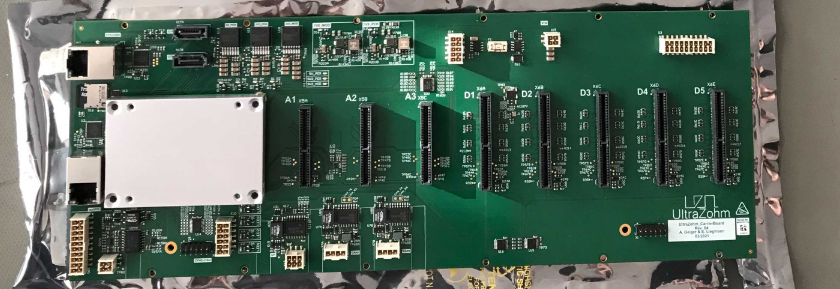
\includegraphics[width=10cm]{ASSETS/UltraZohms_assembled_one.png}
\end{center}


\textbf{1. Passive Test - Perform a visual inspection}\\
\setlist{noitemsep}
\begin{todolist}
\item Are all parts correctly placed or are some of the parts displaced? \\
\item Does it look like anything is missing? \\
\item Is too much solder paste applied and are thus any pins shorted?\\
\end{todolist}

\textbf{2. Passive Test - Measure resistance}\\

\setlist{noitemsep}
\begin{todolist}
\item Measure the ohmic resistance with a multimeter. Please note the real values. \\
\item All of them should be in the range of kOhm. Are all values in the expected range? \\
\end{todolist}

The following measuring points are relevant: \\

\begin{tabular}[h]{l|c|c|c|c}
What & Point 1 & Point 2 & Expected value & Real value \\
\hline
\textcolor{red}{V\_IN} to \textcolor{magenta}{GND} & \textcolor{red}{X14 Pin 1 or 2} & \textcolor{magenta}{X14 GND} & 50-100 kOhm &   \\
\hline
5V\_PER to \textcolor{magenta}{GND} & \textcolor{blue}{TP71} & \textcolor{magenta}{X14 GND} & $>$10 kOhm &   \\
\hline
3V3\_PER to \textcolor{magenta}{GND} & \textcolor{blue}{TP70} & \textcolor{magenta}{X14 GND} & $>$1 kOhm &   \\
\hline
3V3\_MOD to \textcolor{magenta}{GND} & \textcolor{blue}{TP69} & \textcolor{magenta}{X14 GND} & $>$1 kOhm &   \\
\hline
5V\_PER to 3V3\_PER & \textcolor{blue}{TP71} & \textcolor{blue}{TP70} & $>$10 kOhm &   \\
\hline
5V\_PER to 3V3\_MOD & \textcolor{blue}{TP71} & \textcolor{blue}{TP69} & $>$2 kOhm &   \\
\hline
3V3\_PER to 3V3\_MOD & \textcolor{blue}{TP70} & \textcolor{blue}{TP69} & $>$2 kOhm &   \\
\hline
1V8\_PER to \textcolor{magenta}{GND} & \textcolor{blue}{TP78B} & \textcolor{magenta}{X14 GND} & $>$4 kOhm &   \\
\hline
1V8\_MOD to \textcolor{magenta}{GND} & \textcolor{blue}{TP78A} & \textcolor{magenta}{X14 GND} & $>$4 kOhm &   \\
\end{tabular}

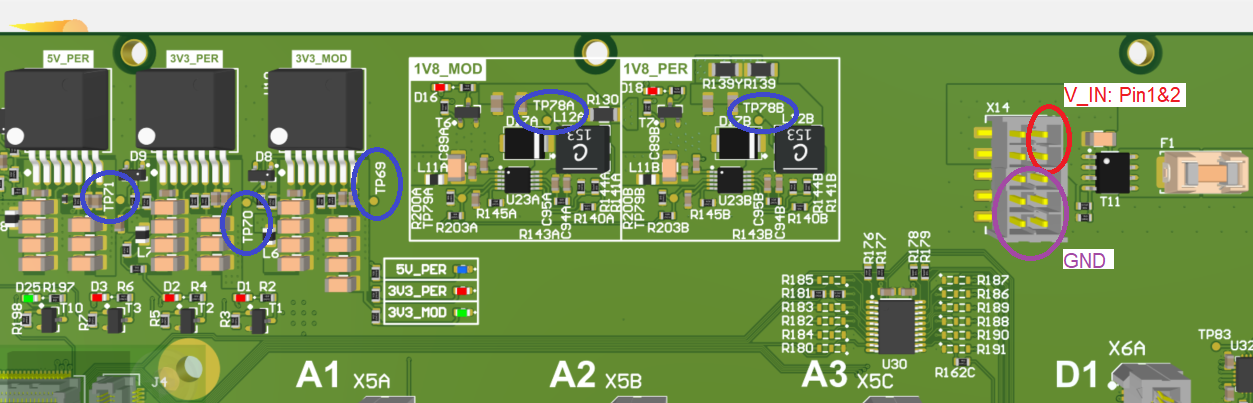
\includegraphics[width=16cm]{ASSETS/Carrier_PowerSupply.png}


\newpage
\textbf{3. Active Test - Measure voltages}

\setlist{noitemsep}
\begin{todolist}
\item First configure the dip switches on the back panel.\\
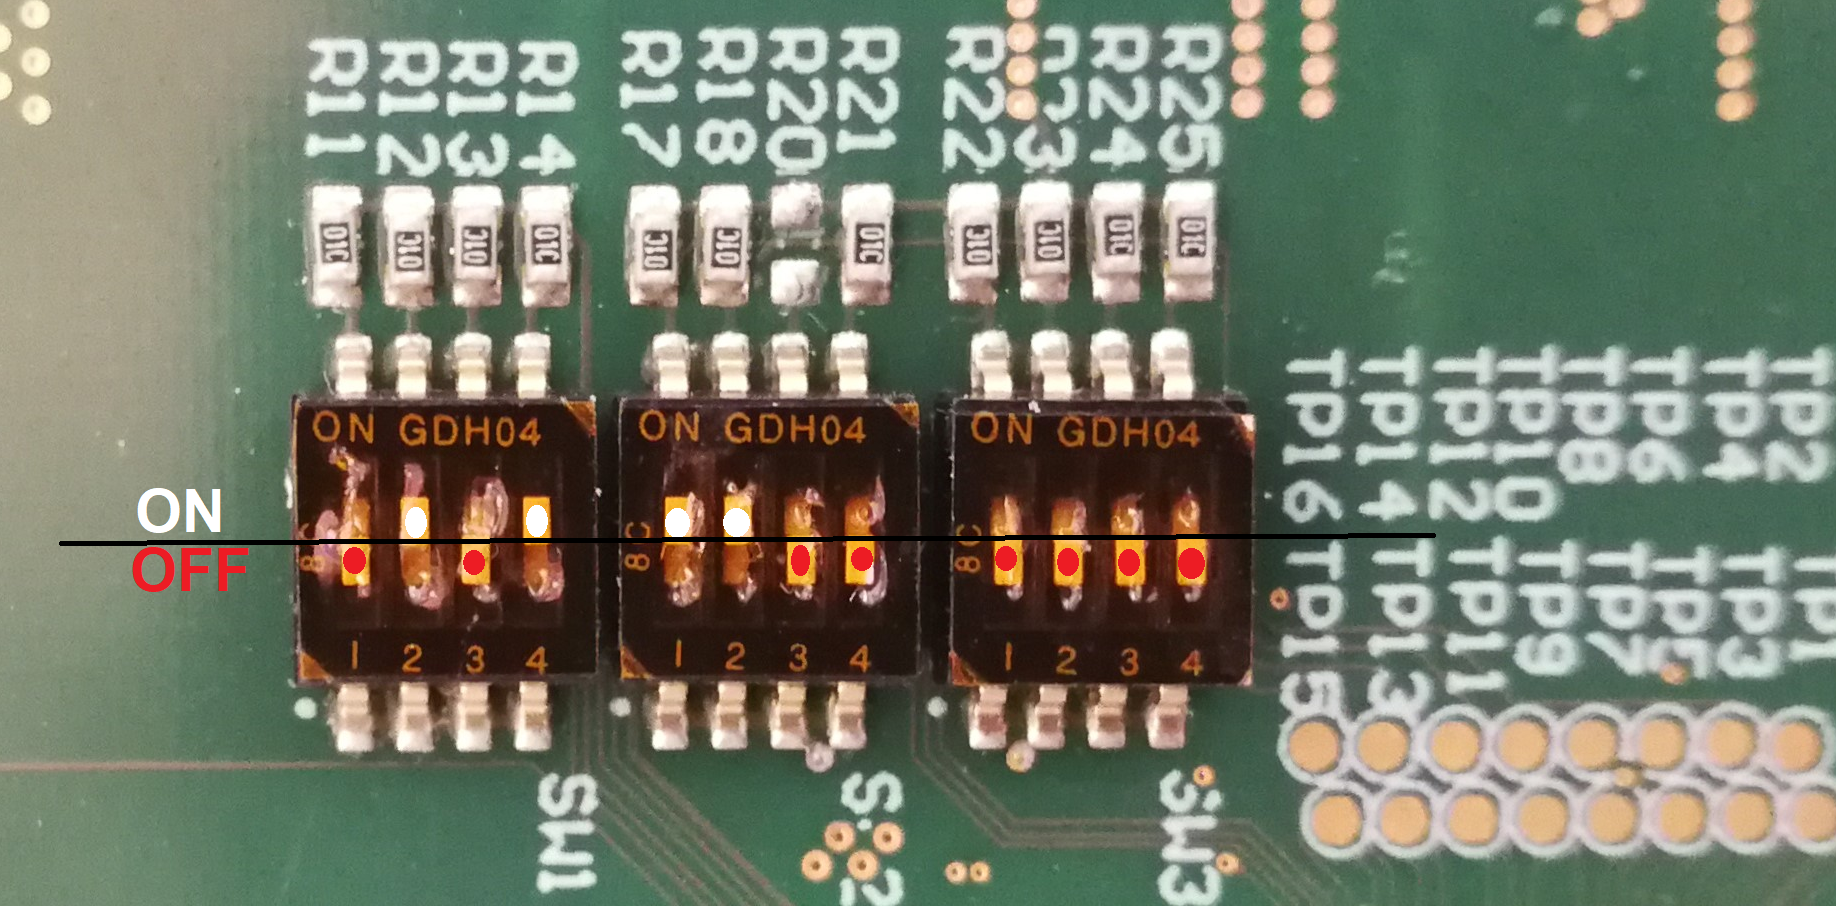
\includegraphics[width=13cm]{ASSETS/Carrier_DipSwitch.png}\\

\item Connect the power supply cable on X14 and supply it with 24\,V @ 300\,mA current limit. A current consumption of around 80-90\,mA is expected. Is this achieved?\\

\item The five LEDs for the five power supply stages are ON?\\
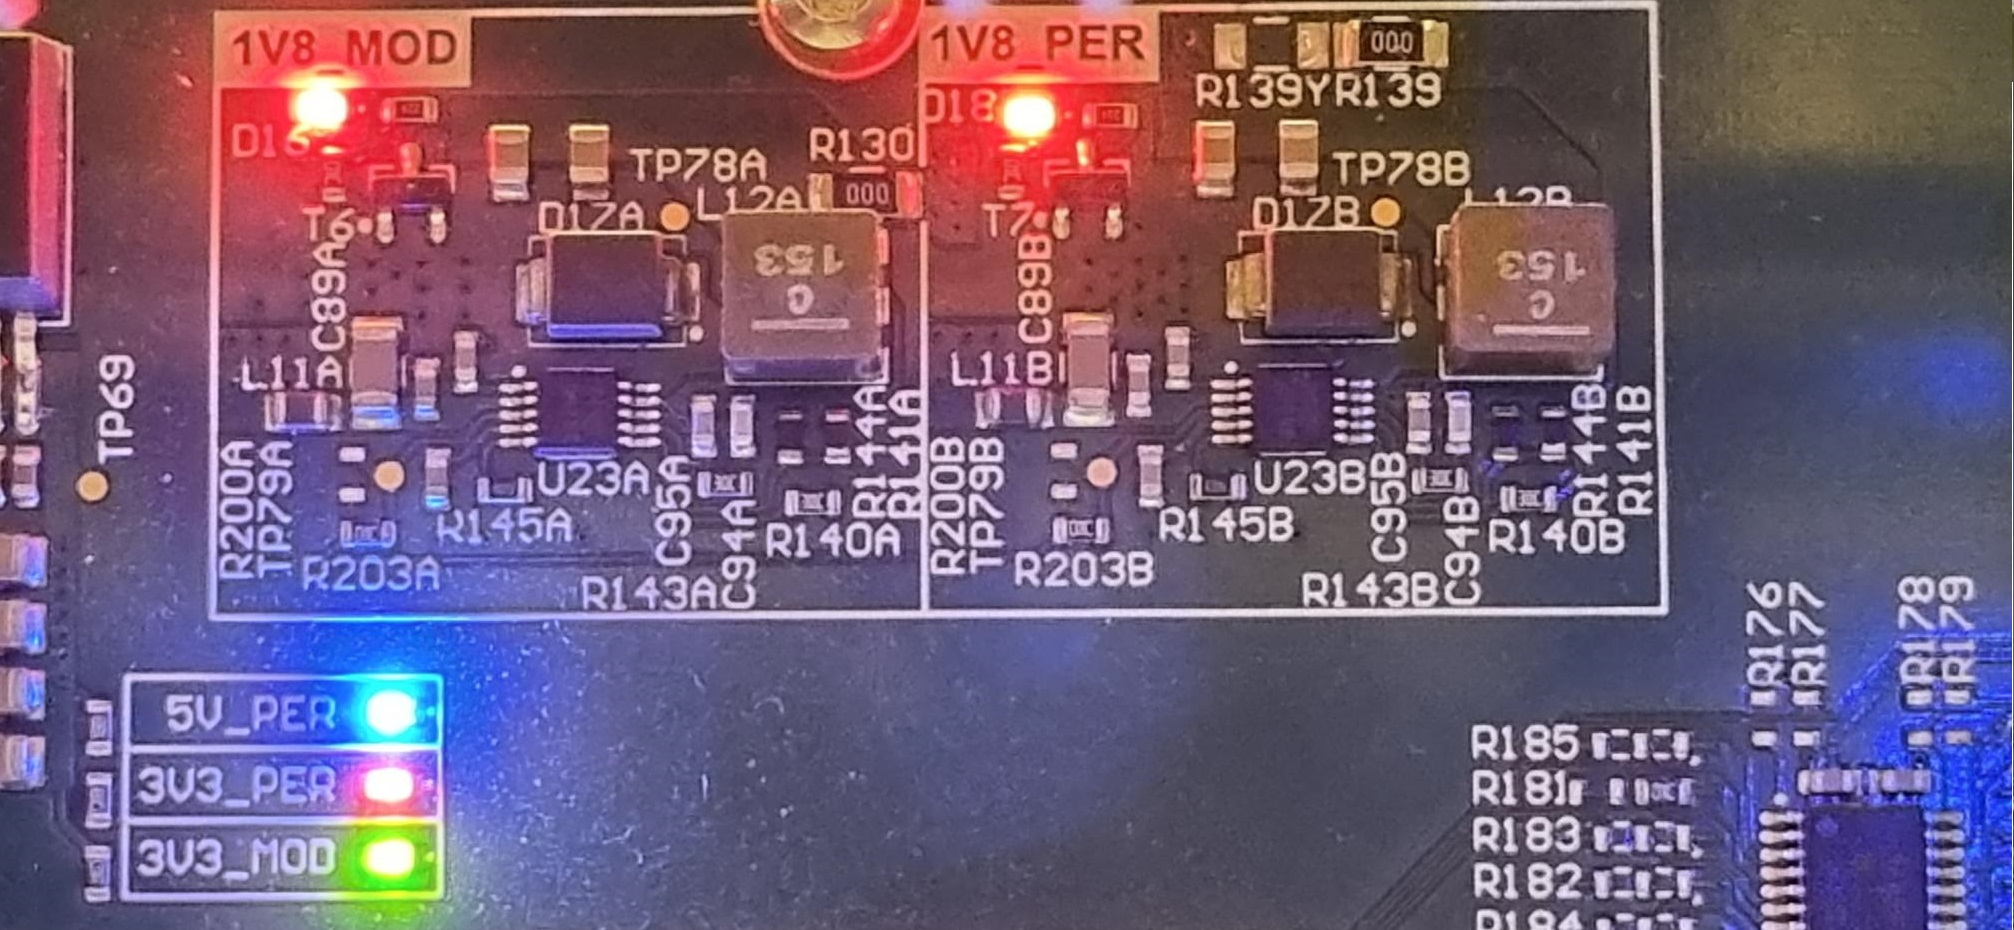
\includegraphics[width=13cm]{ASSETS/Carrier_LED.jpg}\\

\item Measure the supply voltage and the voltage of the five subsequent power supply stages with a multimeter. Are all six voltages inside the expected range?
\end{todolist}

\begin{tabular}[h]{l|c|c|c|c}
What & Point 1 & Point 2 & Expected value & Real value \\
\hline
\textcolor{red}{V\_IN} to \textcolor{magenta}{GND} & \textcolor{red}{X14 Pin 1 or 2} & \textcolor{magenta}{X14 GND} & 24\,V &   \\
\hline
5V\_PER to \textcolor{magenta}{GND} & \textcolor{blue}{TP71} & \textcolor{magenta}{X14 GND} & 4.9 - 5.1\,V &   \\
\hline
3V3\_PER to \textcolor{magenta}{GND} & \textcolor{blue}{TP70} & \textcolor{magenta}{X14 GND} & 3.2 - 3.4\,V  &   \\
\hline
3V3\_MOD to \textcolor{magenta}{GND} & \textcolor{blue}{TP69} & \textcolor{magenta}{X14 GND} & 3.2 - 3.4\,V  &   \\
\hline
1V8\_PER to \textcolor{magenta}{GND} & \textcolor{blue}{TP78B} & \textcolor{magenta}{X14 GND} & 1.75 - 1.85\,V  &   \\
\hline
1V8\_MOD to \textcolor{magenta}{GND} & \textcolor{blue}{TP78A} & \textcolor{magenta}{X14 GND} & 1.75 - 1.85\,V &   \\
\end{tabular}

\newpage
\textbf{4. Active Test - Check the terminal output}

\setlist{noitemsep}
\begin{todolist}
\item Connect a JTAG module TE0790-03 to X8. Check if the JTAG dip switches are set correctly (see picture). Make sure that the SD card is inserted in X16. Connect a USB cable between JTAG module and your laptop.\\  

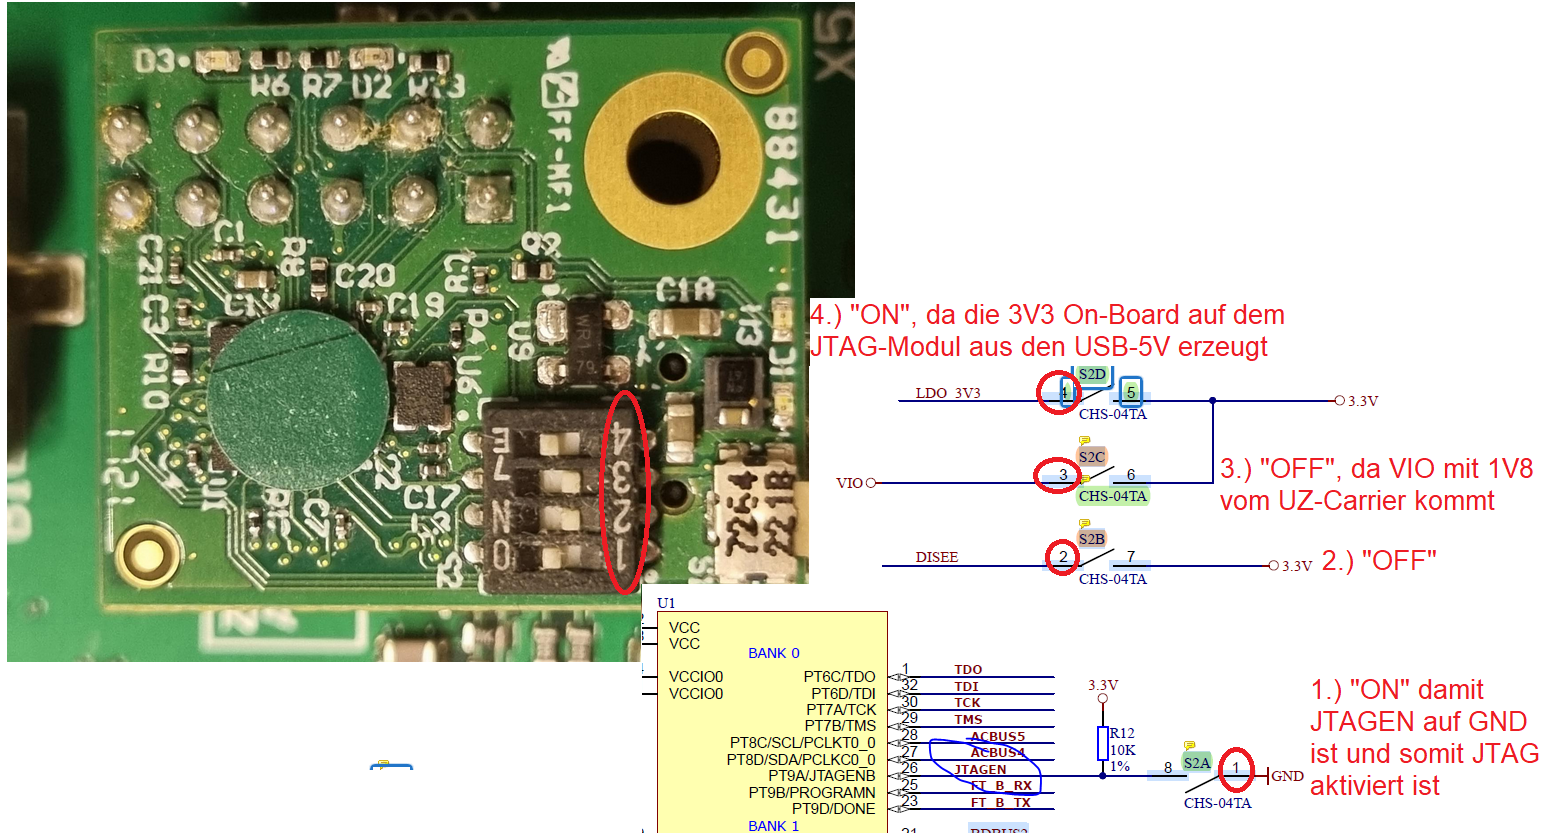
\includegraphics[width=16cm]{ASSETS/Carrier_JTAG.png}

\item Open a terminal, e.g. Tera Term, and connect the serial COM port. Switch on the power supply of the carrier board. Is the FSBL successfully loaded?\\

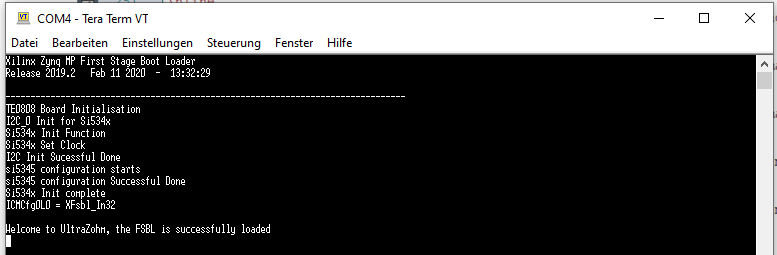
\includegraphics[width=13cm]{ASSETS/Carrier_FSBL.png}

\end{todolist}




\textbf{5. Active Test - Check PHY and Ethernet}

The SD card contains a boot image to test the PHY of the Ethernet. The boot image does the following: 
\begin{itemize}
    \item It loads a FreeRTOS into an A53 core
    \item It looks for the PHY at the MDIO interface and outputs the following status via the on board LEDs:
    \begin{itemize}
    	\item LED 1 must be always on
    	\item LED 2 = netif\_link\_being\_up $\Rightarrow$ ON means the PHY is working
    	\item LED 3 = LED 4 = no PHY detected $\Rightarrow$ ON means ERROR on the PHY
    	\item The photo shows for the PHY the error case:
    	\item 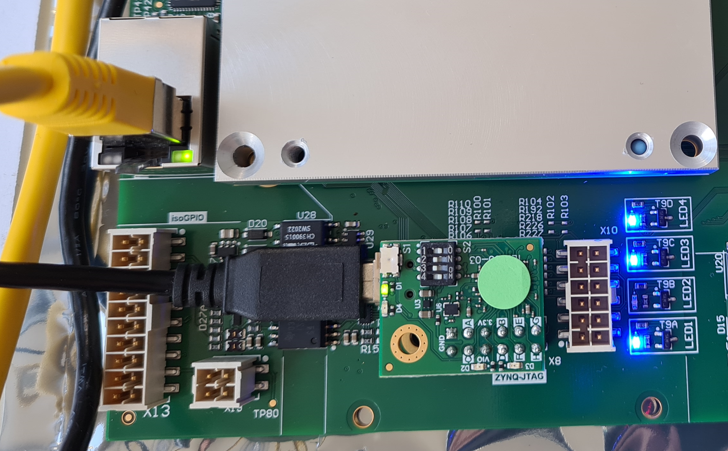
\includegraphics[width=10cm]{ASSETS/PHY_Error_Case.png}
    \end{itemize}
    \item The same information is also output via the UART (on X8). 
    \begin{itemize}
        \item 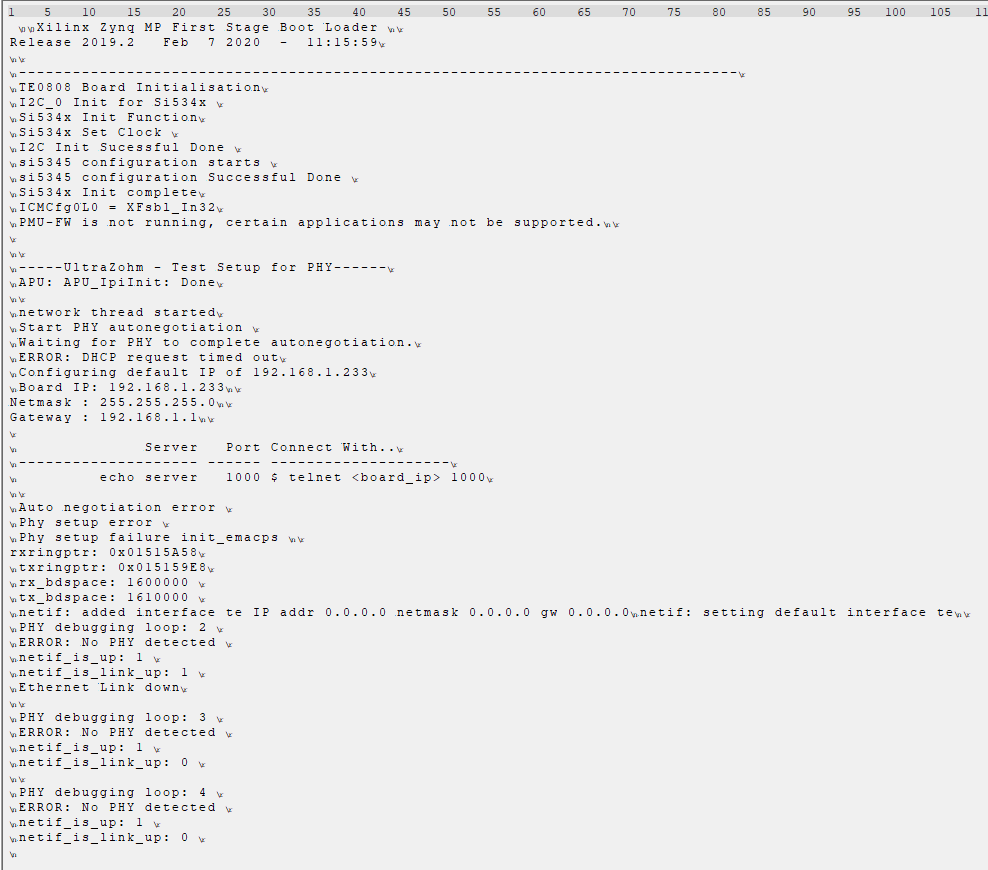
\includegraphics[width=9cm]{ASSETS/PHY_Error_Case_UART.png}
    	\item The UART output occurs approx. every 20 seconds, with this frequency also the function detect\_phy() is called and there should be traffic on the MDIO line.
    	\item Our guess is, that if the PHY is not working, that something is wrong with the MDIO MDC configuration line.
    	\item Schematic and assembly drawing can be found here: 
    	\href{https://docs.ultrazohm.com/hardware/carrier_board/carrier_board_rev04/overview.html#downloads}{www.docs.ultrazohm.com}
    	\item We have 2 PHYs connected to the same MDIO line, this should not be a problem since it works for other boards already sucessfully.
    	\item R240 and R241 disconnect the second PHY from the MDIO line.
    	\item R154 and R155 are optional resistors to insert additional termination.
    \end{itemize}
\end{itemize}

\textbf{6. Property rights}\\

All rights reserved by the UltraZohm community.\\


\textbf{7. Final Provisions}\\

If any of the preceding tests are not successfully passed, the carrier board (TEC0194) is not functional and must either:
\begin{itemize}
    \item The corresponding error must be detected and eliminated. The test procedure must then be performed once again.
    \item If the error cannot be detected or eliminated, the board must be discarded and cannot be shipped.
\end{itemize} 
 
% Grußformel bei einem Namen/Unterschrift
%\closing{Mit freundlichen Grüßen}

% Schlussformel bei mehreren Namen/Unterschriften
\closing{ }%


\end{letter}

% Weitere PDFs können automatisch angefügt werden, z.B. Ahnänge.
%\includepdf[pages=-,openright]{pfad/zu/weiteren/pdfs/dokument.pdf}
% Pfad ist relativ zu dieser tex-Datei. Mit .. ein Verzeichnis hoch.
% Der pages-Parameter spezifiziert welche Seiten eingefügt werden.
% Beispiele:
% pages=-				alle Seiten
% pages={1-4}			Seite 1-4
% pages={1,4,5}			Seite 1, 4 und 5
% pages={3,{},8-11,15}	Seite 3, leere Seite, Seite 8-11 und Seite 15
% Der openright-Parameter startet die Anlagen auf ungerader (rechter) Seite, d.h. notfalls wird eine leere Seite
% eingefügt. Im doppelseitigem Druck wird dadurch besser zwischen Brief und Anlage getrennt. Für einseitigen Druck
% entfernen.



\end{document}
